\documentclass{jsarticle}
\usepackage[margin = .7in]{geometry}
\usepackage[dvipdfmx]{graphicx}
\usepackage{listings}
\usepackage{amsmath}
\usepackage{bm}
\usepackage{ascmac}
\lstset{%
  language={python},
  basicstyle={\small},%
  identifierstyle={\small},%
  commentstyle={\small\itshape},%
  keywordstyle={\small\bfseries},%
  ndkeywordstyle={\small},%
  stringstyle={\small\ttfamily},
  frame={tb},
  breaklines=true,
  columns=[l]{fullflexible},%
  numbers=left,%
  xrightmargin=0zw,%
  xleftmargin=3zw,%
  numberstyle={\scriptsize},%
  stepnumber=1,
  numbersep=1zw,%
  lineskip=-0.5ex%
}

\begin{document}
\title{卒論テーマ候補 :ゆびすま2}
\author{池上 慧}
\maketitle

\section{ゲームの概要}
\subsection{ゆびすまとは}
「ゆびすま」とは2人以上で行われるゲームである。ここでは2人で行われるケースを想定する。プレイヤーは「攻め」と「守り」の役目を交互に行う。プレイヤーは毎回好きな本数の親指を上げる。「攻め」のプレイヤーは今回上がる親指の本数を予想し、その予想した数をコールしながら、自分でも好きな本数だけ親指を上げる。「守り」のプレイヤーも掛け声と同時に親指を好きな本数だけあげる。「攻め」がコールした数と実際にあげられた親指の総数が等しかったなら「攻め」の勝ちであり、そうでなければ「引き分け」である。引き分けたら役割を交代してどちらかが勝つまで続けるものとする。本来であれば勝てば腕を一本減らすことができ、先に二回勝利した方の勝ちというルールであるが、ここでは最初の2本vs2本の状況のみを想定する。

\subsection{ゲームの構造}
このゲームで勝敗を決するのは攻め手が決定する「宣言」と「指」との差である。この差で攻め手の行動を分類することができる。すなわち相手の上げる指の数が0本の時勝利する行動の組である$\left\{ (0,0), (1,1), (2,2)\right\}$をset1とし、相手の指の数が1本の時に勝利する行動の組である$\left\{ (1,0), (2,1), (3,2)\right\}$をset2、相手の指の数が2本の時に勝利する行動の組である$\left\{ (2,0), (3,1), (4,2)\right\}$をset3とする。これを用いてゲームの利得表は以下のように与えられる。
\begin{figure}[h]
    \centering
    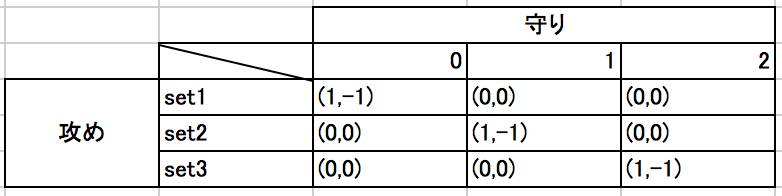
\includegraphics[width=10cm]{pmat.png}
    \caption{利得表}
\end{figure}
2人対称ゼロサムゲームとなる。守り手が$\left\{ 0,1,2\right\}$をそれぞれ取る確率を$(q,r,s)$で表記し、攻め手が取るsetに対しての混合戦略、すなわちset1, set2, set3をとる確率を$(x,y,z)$で表記する。この時の混合戦略ナッシュ均衡は以下のようである。
\begin{itembox}[l]{case1 : 完全に合理的な主体を想定したナッシュ均衡}
    \begin{align}
    	\begin{cases}
		(q, r, s) = (\frac{1}{3}, \frac{1}{3}, \frac{1}{3})\\
		(x, y, z) = (\frac{1}{3}, \frac{1}{3}, \frac{1}{3})
	\end{cases}
    \end{align}
\end{itembox}

つまり攻め手も守り手も自身の行動に等しく確率を割り振るのが最適反応を構成している。この時攻め手の本来の行動である$9$個の「宣言」と「指」のペアに対しても等しく$\frac{1}{9}$ずつ確率が振られている。

\section{研究の目的意識}
しかし上記のように全ての戦略に等しく確率を割り振る戦略が実際のプレイでは取られていない可能性が高い。$[a,b]$で宣言$a$ゆびの数$b$の攻め手の行動を表すことにすると、経験的には$[2,1]$のようなある種中途半端な戦略が$[0,0]$や$[4,2]$のような極端な戦略よりも取られやすい傾向があるようように思える。実際、地域によっては利得構造は変えずに$[0,0]$と$[4,2]$に対して特別な名称を与え、他の行動とは別物として扱われているようである。

限定合理性のモデル化によって上記の現象が説明できないかを考える。2人完備情報ゲームに適用可能な限定合理生のモデルとして代表的なものにはOsborn and Rubinshtein (1998)で提案されたS(k) EquilibriumやMcKelvey and Palfrey (1995)で提案されたquantal response equilibriumなどがある。しかし、先に挙げたこのゲームの利得表を見ればわかる通りゆびすまは対称なゲームである。このような単純な構造を持つゲームにおいて特定の行動が特別選ばれがちになるような限定合理生のモデルは既存のモデルには見当たらず、実際上記の二つの計算結果は先のナッシュ均衡と同じになってしまう。

ここではこの現象を説明する方向性として、ゲームの基幹とも言える行動主体とその取りうる行動に関する認識自体が完全ではない時にどのような行動がとられるかを分析する。具体的には以下の二つの軸でゲームの構造への誤認が発生している状況を考える。
\begin{enumerate}
	\item 相手主体を分割し異なる複数主体が相手の手を構成しているかのように誤認する(擬人化)
	\item 複数要素の組み合わせで表現される自身の行動を組み合わせそのものとして捉えることができず個別要素ごとに最適行動を取ろうとする(統合失敗)
\end{enumerate}

ゆびすまにおいて具体的に見ていく。本来は$\left\{ 0,1,2 \right\}$である守り手の行動について誤認が発生するのが一つ目の非合理性であり、そこでは相手のゆびがそれぞれ別の主体によって動かされているという想定の下行動することになる。すなわち本来2人ゲームであるゆびすまを3人ゲームであるかのように振舞うことになる。ゆびすまにおいてこのような誤認が発生しうるであろう根拠としてはゲームの進行にしたがって指が1本ずつ減らされていくという点が挙げられる。今回の研究ではこの2本vs2本の状況しか扱わないが、ゆびすまは広く知られたゲームであるためこの認識はどのプレイヤーにも浸透していると考えられる。

一方で、攻め手が「宣言」と「指」の組み合わせとして自身の行動が決まっているという認識を正しく持てない状況が二つ目の非合理性である。「宣言」を縦軸に、「指」を横軸にした表の上で攻め手の行動を考える。
\begin{figure}[h]
    \centering
    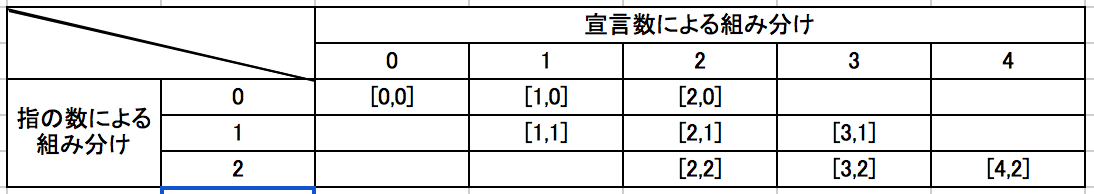
\includegraphics[width=10cm]{class2.png}
    \caption{組み分け}
\end{figure}
まず、自身の行動を組み合わせとして正しく認識しているということが何を指すのかを考える。組み合わせとして正しく認識しているとは、図1のような利得表がこのゲームの利得表であるということを正しく認識した上でゲームをプレイするということである。すなわち先に述べたset1からset3がそれぞれ同じ勝利条件であることを認識し、setごとに混合戦略の確率を振ることができる状況である。図2の表でいうと、$9$個の組み合わせに対して斜めに3個ずつのグループ分けをしている状況である。

しかし「宣言」と「指」の組み合わせに対してどれが無差別となるかを正しく認識してプレイするのは人間には難しすぎる(気がする)。瞬時にプレイすることを求められた時にプレイヤーができることは、「勝ちやすい宣言」と「勝ちやすい指」とを組み合わせるのがせいぜいであろうと考えられる。よって「宣言」と「指」を別々の行動と見てそれぞれで勝ちやすい行動をとった結果として何らかの組み合わせが行動としてプレイされているのであるとして行動を分析する。

ただし、「宣言」と「指」について別々に行動の確率を割り振ることができないことには注意が必要である。最低限頭が使えれば$[0,1]$のような勝利確率が$0$となる行動を攻め手がとらないことは明らかである。すなわちそのような行動に対しては確率$0$を割り振るべきだということになる。仮に「宣言」と「指」に別々の混合戦略を与えてしまうと、図2において空欄となっている完全に非合理な行動に対しても何らかの正の確率が振られることになる。また、これを回避しようすると、「宣言」においては$0,4$を、「指」においては$0,2$をとらないという戦略しか取れなくなる。これでは、確かに先に述べたような$[2,1]$などの中途半端な行動は取りうるが、$[0,0, [4,2]]$といった極端な行動をとらないことになってしまう。現実にはそのような行動も取られるため、バランスよく偏った行動をプレイヤーが取るためには「宣言」と「指」に別々の確率を割り振ってはいけないということになる。

そこで、「宣言」について条件付けた「指」への条件付き混合戦略を考えることとする。すなわち「宣言」である$(0,1,2,3,4)$に対して割り振る確率$(p_0,p_1,p_2,p_3,p_4)$と、宣言$i$の時に指$j$に割り振る確率$\left\{ a_i^j \right\}_{i = 0,1,2,3,4}^{j = 0,1,2}$とについて最適な行動をとるように考える。

上記の二つの非合理性の組み合わせから以下の4つのモデルから行動の帰結を得て、どのモデルが実験データに最もフィットするかを統計的検定を用いて判断し、ゆびすまゲームにおける非合理性の現出の仕方を明らかにするのが目的である。

\begin{description}
	\item[モデル1] 完全に合理的主体
	\item[モデル2] 非合理性1のみ存在
	\item[モデル3] 非合理性2のみ存在
	\item[モデル4] 非合理性1,2の両方が存在
\end{description}

\section{モデルの帰結}
\subsection{モデル1}
先に示したナッシュ均衡をモデルの予測とする。すなわち全ての手を等しい確率で取る。

\subsection{モデル2}
先に述べた非合理性$1$の下での混合戦略ナッシュ均衡は以下の三つが計算できる。ただし$p$は一つの指が上がる確率である。
\begin{itembox}[l]{モデル2の均衡}
\begin{align}
    	&\begin{cases}
		p = \frac{1}{3}\\
		(x, y, z) = (\frac{1}{3}, \frac{2}{3}, 0)
	\end{cases}\\[10pt]
	&\begin{cases}
		p = \frac{1}{2}\\
		(x, y, z) = (0, 1, 0)
	\end{cases}\\[10pt]
	&\begin{cases}
		p = \frac{2}{3}\\
		(x, y, z) = (0, \frac{2}{3}, \frac{1}{3})
	\end{cases}
\end{align}
\end{itembox}
上から均衡$1,2,3$と呼ぶことにする。この時、均衡$1,3$での攻め手の期待利得、すなわち勝利確率は$\frac{4}{9}$であり、均衡$2$における攻め手の勝利確率は$\frac{1}{2}$である。ゆびすまはゼロサムゲームであるので、この大小関係は守り手の敗北確率に直結する。今考えている非合理性の下では各ゆびが別々に意思決定をしていると攻め手が勝手に思い込んでいるので、守り手の敗北確率が低くなるように守り手が戦略をとるだろうと勝手に想定することになる。この思い込みの下では均衡$2$は実現しないと想定することになる。よって、非合理性$1$の下で攻め手がとる行動の予測としては、均衡$2,3$が得られる。

\subsection{モデル3}
先に述べた通り、上げる指の数に対しては宣言数に条件付けた混合戦略を、宣言数については通常の混合戦略を考える。図$2$からゲームの構造に対称性が存在することは明らかであり、考えるべき要素は$(p_0,p_1,p_2),$と$(a, b)$の5つに絞れる。ここで$p_0$は$0$か$4$を宣言する確率、$p_1$は$1$か$3$を宣言する確率、$p_2$は$2$を宣言する確率である。また、$a$は宣言が$1$の時に指を$0$本あげる確率であるとともに宣言が$3$の時に指を$2$本あげる確率で、$b$は宣言が$2$の時に指を$0$本あげる確率であるとともに$2$の時に指を$2$本あげる確率である。ここで$2p_0 + 2p_1 + p_2 = 1$であることを考慮すると、通常の意味で確率が定式化されるために以下の制約が必要である。
\begin{align}
\begin{cases} 
p_0 + p_1 \leq \frac{1}{2}\\[7pt]
0 \leq a \leq 1\\[7pt]
0\leq b \leq \frac{1}{2}
\end{cases}
\end{align}
この制約を考慮した時に、このモデルの帰結として得られる行動予測を計算すれば良い。

このモデルを解くために以下のゲームを考える。乱数で発生させた「宣言」を攻め手のみが知っている状態でゆびすまをプレイさせる。このゲームは不完備情報ゲームとなり、ベイジアンナッシュ均衡を求めることができる。この時ベイジアンナッシュ均衡を構成するのは、攻め手の各宣言数で条件付けられた時の指の上げ下げについての混合戦略と守り手の混合戦略である。このように自然な形で先に述べた条件付きの混合戦略を考えることができるのでこの形式での解を求めることに意味がある。

守り手が指を$0,1,2$本あげる確率を$(r_0, r_1, r_2)$として表記すると、ベイジアンナッシュ均衡は以下である。
\begin{itembox}[l]{宣言数を乱数で発生させた時のベイジアンナッシュ均衡}
\begin{align}
\begin{cases}(r_0^*, r_1^*, r_2^*) = (\frac{1}{3}, \frac{1}{3}, \frac{1}{3}) \\[7pt]
(a^*, b^*) \in \left\{ (a,b) \mid 0 \leq a \leq 1, 0 \leq b \leq \frac{1}{2}\ \right\}
\end{cases}
\end{align}
\end{itembox}
これはすなわち、守り手が$(\frac{1}{3}, \frac{1}{3}, \frac{1}{3})$という戦略を取る限り、宣言数について条件付けた指の上げる数の混合戦略はどのようなものにしても最適反応となるということを意味している。また、この均衡において攻め手は自身の宣言数(タイプ)に依存した戦略をとらなくても最適反応であることにも注意が必要である。この事実より、モデル3においてモデルが予測する均衡は、
\begin{itembox}[l]{モデル3の帰結}
\begin{align}
\begin{cases}(r_0^*, r_1^*, r_2^*) = (\frac{1}{3}, \frac{1}{3}, \frac{1}{3}) \\[7pt]
(p_0^*, p_1^*) \in \left\{ (p_0, p_1) \mid 0 \leq p_0 + p_1 \leq \frac{1}{2}, 0 \leq p_0, 0 \leq p_1 \right\}\\[7pt]
(a^*, b^*) \in \left\{ (a,b) \mid 0 \leq a \leq 1, 0 \leq b \leq \frac{1}{2}\ \right\}
\end{cases}
\end{align}
\end{itembox}
として得られる。すなわち、制約$(5)$を満たす混合戦略の組は全て守り手の取る$(r_0^*, r_1^*, r_2^*)$に対する最適反応であることになる。


\subsection{モデル4}
ここでもモデル3と同様に、まず宣言についての確率分布を固定してベイジアンナッシュ均衡を計算する。モデル3と同様の対称性の過程を置いた時に以下の4つがベイジアンナッシュ均衡として得られる。ただし$q$は守り手の指が上がる確率であり、$a,b$に関してはモデル3と同様である。
\begin{itembox}[l]{モデル4の均衡}
\begin{align}
&(q, a, b) = \left(\frac{1}{2},\ 1,\ 0\right)\\[7pt]
&(q, a, b) = \left(\frac{3 - \sqrt{3}}{6},\ 0,\ \frac{1}{4} - \frac{1}{4}\left( \frac{1-p_2}{p_2} \right) \right)\\[7pt]
&(q, a, b) = \left( \frac{1}{3},\ 1 + \frac{6p_0 - 2}{6p_1},\ 0 \right)\\[7pt]
&(q, a, b) = \left( \frac{3 + \sqrt{3}}{6},\ 1,\ \frac{1 - 3p_0}{3p_2} \right)
\end{align}
\end{itembox}
ただし均衡$(8)$を除いて$(p_0, p_1)$の値に依存して均衡の存在する範囲が決まっていることに注意する。この範囲に注意しながら、モデル2の時と同様に、守り手が攻め手の勝利確率を最小化していると攻め手が想定した時に、最小化された勝利確率を最大化するように宣言の確率分布を決定することでこのモデルの帰結を得るとする。これによって導かれるモデルの帰結は以下である。
\begin{itembox}[l]{モデル4の帰結}
\begin{align}
\begin{cases}
&(p_0, p_1) \in \left\{ (p_0, p_1) \mid \frac{1}{4} \leq p_0 \leq \frac{1}{3}, \frac{1}{3} -p_0 \leq p_1 \leq \frac{1}{2} - p_0 \right\}\\[6pt]
&(q, a, b) = \left( \frac{1}{3},\ 1 + \frac{6p_0 - 2}{6p_1},\ 0 \right)
\end{cases}
\end{align}
\end{itembox}


\end{document}



































